156. \begin{figure}[ht!]
\center{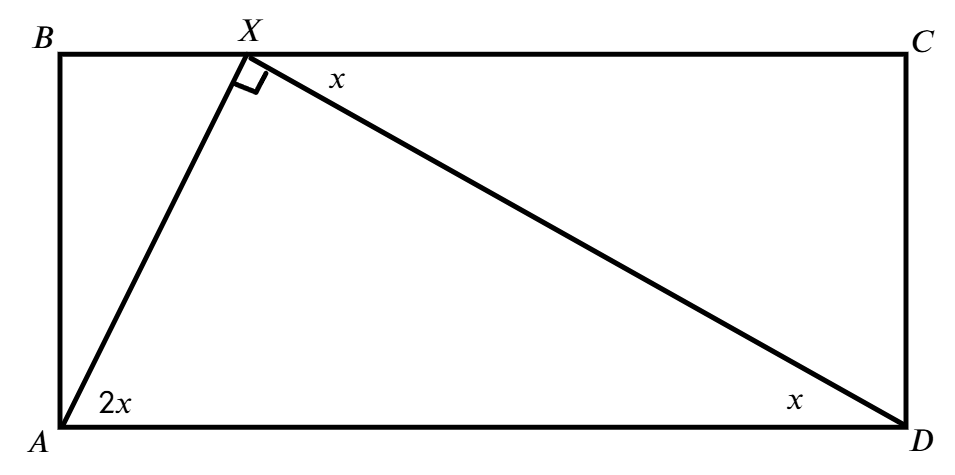
\includegraphics[scale=0.35]{g7-153.png}}
\end{figure}\\
Углы $CXD$ и $XDA$ равны как накрест лежащие. Обозначим $\angle CXD=\angle XDA=x,$ тогда $\angle XAD=2x$ и из треугольника $AXD$ получим равенство $x+2x+90^\circ=180^\circ,$ откуда $x=30^\circ,\ 2x=60^\circ.$ Тогда $\angle BAX=90^\circ-60^\circ=30^\circ$ и по теореме о катете, лежащем напротив угла в $30^\circ,$ для треугольника $ABX$ получим соотношение $AX=2BX.$ По той же теореме для треугольника $AXD$ получим соотношение $AD=2AX=4BX.$ Тогда $XC=BC-BX=AD-BX=4BX-BX=3BX,$ таким образом $BX:XC=1:3.$\newpage\noindent
